\documentclass[10pt,a4paper]{article}
\usepackage[toc,page]{appendix}
\usepackage[margin=2.4cm]{geometry} % margins
\usepackage{amsmath}
\usepackage{bm} % for bold math
% \usepackage{textgreek}
\usepackage{graphicx}
\usepackage[labelfont=bf,nooneline]{caption} % for subfigs %font=small
\usepackage{subcaption} % for subfigs
\usepackage{hyperref} % hyperlinks [colorlinks=true]
\usepackage{booktabs} % spaces between columns
\usepackage{cancel} % MET: $\cancel{\it{E}}_{T}$
\setlength{\tabcolsep}{7pt}

\newcommand{\cc}[1]{\multicolumn{1}{c}{#1}} % centered cell
\newcommand{\levels}[1]{ \multicolumn{2}{l}{\hspace{-1em}\textbf{#1}}}
\newcommand{\level}[1]{ \multicolumn{5}{l}{\hspace{-1em}\textbf{#1}}}
\newcommand{\T}{\rule{0pt}{2.9ex}}       % Top strut
\newcommand{\B}{\rule[-1.3ex]{0pt}{0pt}} % Bottom strut
\newcommand{\ww}{7.7cm} % width for two figures next to each other
%\newcommand{\hh}{1mm} % height between figures above each other
\newcommand{\dd}{-2mm} % distance reduction between one-lined caption and their figure below

\renewcommand{\tt}{$\text{t}\bar{\text{t}}$}
\newcommand{\bbWW}{$\rightarrow$ bbWW}
\newcommand{\di}{$\rightarrow$ bbWW $\rightarrow$ bb$\ell\nu \ell\nu$}
\newcommand{\semi}{$\rightarrow$ bbWW $\rightarrow$ bb$qq\ell\nu$}
\newcommand{\channels}{bbWW $\rightarrow$ bb$\ell\nu\ell\nu$, bb$qq\ell\nu$} % or bbWW $\rightarrow$ bb$qq\ell\nu$ }
\newcommand{\lnu}{$\ell\nu$}
\renewcommand{\ll}{\ell\ell}
\newcommand{\bb}{\text{bb}}
\renewcommand{\sf}{$\sigma_{\text{full}}$}
\newcommand{\sAN}{$\sigma_1$}
\newcommand{\BR}{\mathcal{B}}
\newcommand{\etal}{\emph{et al.}}
\newcommand{\MET}{$\cancel{\it{E}}_{T}$}

\title{Report on comparison between analyses for semi- and dileptonic channels of HH production at HL-LHC}
\author{Izaak Neutelings (University of Zurich)}
%\date{31 maart 2013}

% https://twiki.cern.ch/twiki/bin/view/Sandbox/CMSGuidelinesforAuthors
% https://twiki.cern.ch/twiki/bin/view/Sandbox/CMSGuidelinesforAuthors#Symbols
% https://svnweb.cern.ch/cern/wsvn/tdr2/utils/trunk/general/notes_for_authors.pdf
% http://physics.nist.gov/cuu/pdf/sp811.pdf
% http://mirrors.rit.edu/CTAN/macros/latex/contrib/hepnames/hepnames.pdf

\begin{document}
\maketitle





% Introduction
This reportss compares results of selection level cuts of the analysis of HH \di\ with the analysis note by C. Delaere \etal\ \cite{AN} and a new HH \semi\ analysis.





% Samples
\section{Samples}

The Monte Carlo samples of the analysis note were generated by \textsc{MadGraph\_aMC@NLO}, and the parton shower and hadronization was done in \textsc{Pythia6}. Our samples were fully produced in \textsc{Pythia6}. All samples were finally reconstructed with Delphes for the CMS Phase II technical proposal.
For our analysis, the samples only contain \mbox{bbWW $\rightarrow$ bb\lnu\lnu} or \mbox{bbWW $\rightarrow$ bb$qq$\lnu} at generator level, where taus coming from a W-boson are excluded. %no \mbox{H $\rightarrow$ ZZ} and $\ell = \text{e}, \mu$. %and taus coming from a W are excluded. %The HH-samples do not include H $\rightarrow$ ZZ, like they do for C. Delaere \etal.





% Event selections \& clean-up
\section{Event selections \& clean-up}

To reproduce the results by C. Delaere \etal, the event selections and clean-up as described in their analysis note are applied to our samples. %(The code can be found here: \cite{code_HH} \cite{code_tt}.)
Similar selections are made in the semileptonic case, however note that there are no cuts equivalent to $\Delta R_{\ll}$, $M_{\ll}$ or $\Delta \phi_{\text{bb},\ll}$ at generator or clean-up level for the semileptonic case, leading to bigger differences between the two cases. All cuts are compared in Table \ref{cuts}.





% Cross section
\section{Cross section \& branching ratios}

For our analysis, we have been using the cross sections at $\sqrt{s}=14$ TeV given in Table \ref{sigma}. The analysis note lists next leading order $\sigma_\text{LO}$ with $k$-factor $k_\text{NNLO}$ of the samples, all listed in Table \ref{sigma_AN}. %We calculate back to the full cross section of HH or \tt\ production using
%\begin{equation} \label{sf}
%	\sigma_1 = \frac{k_\text{NNLO}\sigma_\text{LO}}{e\BR}
%\end{equation}
%with the appropriate branching ratio $\BR$. The \tt\ cross section is divided by the filter efficiency of \mbox{$e=0.37$} to account for the $63\%$ loss of events after cuts on our \tt\ sample at generator level.
%For the HH sample, we assume $e=1$, as the analysis not describes no cuts at generator level in this case.

The branching ratios are found using
\begin{align*}
    \mathcal{B}(\text{HH $\rightarrow$ bbWW})
        &= 2\mathcal{B}(\text{H $\rightarrow$ bb})
            \mathcal{B}(\text{H $\rightarrow$ WW})
        \simeq 0.248 \\
    \mathcal{B}(\text{\tt\ $\rightarrow$ bWbW})
        &= \mathcal{B}(\text{t $\rightarrow$ bW})^2
        \simeq 0.997 \\
%              0,9966 CDF 2014
%              0,8281 PDG 2014
    \mathcal{B}(\text{WW $\rightarrow$ \lnu\lnu})
        &= \mathcal{B}(\text{W $\rightarrow$ \lnu})^2
        \simeq 0.046 \\
    \mathcal{B}(\text{WW $\rightarrow qq$\lnu})
        &= 2\mathcal{B}(\text{W $\rightarrow$ $qq$})
            \mathcal{B}(\text{W $\rightarrow$ \lnu})
        \simeq 0.288
\end{align*}
with numbers from \cite{BR_HH}, \cite{BR_tt} and \cite{BR_W}:
\begin{align*}
    \mathcal{B}(\text{HH $\rightarrow$ bbWW $\rightarrow$ bb\lnu\lnu})
         &\simeq 0.011\\
%        &= 2\mathcal{B}(\text{H $\rightarrow$ bb})
%            \mathcal{B}(\text{H $\rightarrow$ WW})
%            \mathcal{B}(\text{W $\rightarrow \ell\nu$})^2 \\
    \mathcal{B}(\text{HH $\rightarrow$ bbWW $\rightarrow$ bb$qq$\lnu})
         &\simeq 0.072\\
%        &= 2\mathcal{B}(\text{H $\rightarrow$ bb})
%            \mathcal{B}(\text{H $\rightarrow$ WW})
%            *2\mathcal{B}(\text{W $\rightarrow$ qq})
%            \mathcal{B}(\text{W $\rightarrow \ell\nu$}) \\
    \mathcal{B}(\text{\tt\ $\rightarrow$ bbWW $\rightarrow$ bb$qq$\lnu\lnu})
         &\simeq 0.045\\
%        &=  \mathcal{B}(\text{t $\rightarrow$ bW})^2
%            \mathcal{B}(\text{W $\rightarrow \ell\nu$})^2 \\
    \mathcal{B}(\text{\tt\ $\rightarrow$ bbWW $\rightarrow$ bb$qq$\lnu})
         &\simeq 0.287
%        &=  \mathcal{B}(\text{t $\rightarrow$ bW})^2
%            *2\mathcal{B}(\text{W $\rightarrow$ qq})
%            \mathcal{B}(\text{W $\rightarrow \ell\nu$}) \\
\end{align*}



\begin{table}[p]
	\centering
	\caption{Event selectiona and clean-up: comparison between the dileptonic and semileptonic final state.} \vspace{5pt}
	\label{cuts}
	\begin{tabular}{@{\quad}ll@{}}
	\toprule
	dileptonic final state                     &   semileptonic final state   \\
	\midrule
%	\levels{Gen level} \T\\
%	bbWW$\rightarrow$bb\lnu\lnu  & bbWW$\rightarrow$bbqq\lnu \\
	\levels{Generator level filter on background} \T\\
	b-quarks: $p_T > 15$ GeV                      & b-quarks: $p_T > 15$ GeV    \\
	leptons: $p_T > 15$ GeV, $|\eta| < 2.5$       & lepton: $p_T > 15$ GeV, $|\eta| < 2.5$    \\
	$\Delta R_{\ll} < 2.5$                        & \\%$\Delta R_{q\ell} < 2.5$ \\
	\levels{Selection} \T\\
	two b-tagged jets: $p_T > 30$ GeV, $|\eta|<2.5$ & min. two b-tagged jets: $p_T > 30$ GeV, $|\eta|<2.5$ \\
	                                              & min. four jets: $p_T > 20$ GeV, $|\eta|<2.5$ \\
	two oppositely charged leptons with:          & one lepton with: \\
	\quad muons: $p_T > 20$ GeV, $|\eta|<2.5$     & \quad muon: $p_T > 20$ GeV, $|\eta|<2.5$ \\
	\quad electrons: $p_T > 25$ GeV, $|\eta|<2.5$ & \quad electron: $p_T > 25$ GeV, $|\eta|<2.5$ \\
	\MET $> 20$ GeV                                & \MET $> 20$ GeV \\
	\levels{Clean-up} \T\\
	$60 \text{ GeV} < M_{\bb} < 160 \text{ GeV}$  & $60 \text{ GeV} < M_{\bb} < 160 \text{ GeV}$ \\
	$\Delta R_{\bb} < 3.1 \text{ GeV}$            & $\Delta R_{\bb} < 3 \text{ GeV}$ \\
	$M_{ll} < 85 \text{ GeV}$                     & \\
	$\Delta R_{\ll} < 2$                          & \\
	$\Delta \phi_{\text{bb},\ll} < 1.7$           & \\
%	\bottomrule
	
	\end{tabular}
\end{table}


\begin{table}[p]
	\centering
	\caption{Cross sections at NNLO and $\sqrt{s}=14$ TeV \cite{sigma_HH}\cite{sigma_tt}, branching ratios $\BR$ (excluding W $\rightarrow \tau\bar{\tau}$) \cite{BR_HH}\cite{BR_tt}\cite{BR_W} and number of Monte Carlo events per process in our analysis sample.} \vspace{5pt}
	\label{sigma}
	\begin{tabular}{@{}lccc@{}}
	\toprule
	process      & $\sigma\BR$ [fb] & branching ratio $\BR$ & number of MC events \\
	\midrule
	\textbf{HH}  & \textbf{40}      &           & \\ %\textbf{979 907} \\
	HH \semi     &        2.88      &   0.072   &  166 483  \\
	HH \di       &        0.44      &   0.011   &   22 812  \\
	\bm{\tt}     & \textbf{984 500} &           & \\ %\textbf{499 600} \\
	\tt \semi    &     282 552      &   0.287   &  164 661  \\
	\tt \di      &      44 303      &   0.045   &   22 546  \\
	\bottomrule
	\end{tabular}
\end{table}


\begin{table}[p]
	\centering
	\caption{Cross sections for their Monte Carlo samples listed in the analysis note by C. Deleare \etal\ \cite{AN}.} \vspace{5pt} %and \sAN\ from Eq. \eqref{sf} with a filter efficiency $e=1$ for HH and $e=0.37$ for \tt\ to account for cuts at generator level.
	\label{sigma_AN}
	\begin{tabular}{@{}lcccc@{}}
	\toprule
	process            & $\sigma_\text{LO}$ [fb] & $k_\text{NNLO}$ & number of MC events \\
	\midrule
	HH \di             &  0.163  &   2.3   & 1.1M \\
	\tt\ full leptonic &  9030   &  1.85   & 4.8M \\
%	HH \di             &  0.163  &   2.3   &  33.2   & 1.1M \\
%	\tt\ full leptonic &  9030   &  1.85   & 994 493 & 4.8M \\
	\bottomrule
	\end{tabular}
\end{table}


\begin{table}[p]
	\centering
	\caption{Number of MC events in our sample at each level of selection.} \vspace{5pt}
	\label{raw}
	\begin{tabular}{@{\quad}lrrrr@{}}
	
	\toprule
	               & \multicolumn{2}{c}{dileptonic final state} & \multicolumn{2}{c}{semileptonic final state} \\
	\cmidrule(r){2-3} \cmidrule(r){4-5}
	selection level                      &  signal  & background &  signal  & background \\
	\midrule
% without taus in sample
	\channels				             &  22812  &  22546 & 166483 & 164661 \\
	Generator level filter on background &  22812  &   8339 & 166483 & 137880 \\
	Selection                            &   2571  &   1636 &  28821 &  36760 \\
	Clean-up                             &   2066  &    280 &  22225 &  15300 \\
% with taus in sample
%	Sample without any cuts      &  51464  &  50789 & 214888 & 211952 \\
%	Gen level cuts on background &  51464  &  18899 & 214888 & 101940 \\
%	Selection                    &   3181  &   2023 &  26511 &  20848 \\
%	Clean-up                     &   2499  &    331 &  20634 &   9428 \\
	\bottomrule
	
	\end{tabular}
\end{table}





% Significance and yield
\section{Significance \& yield}

Using the yield $N = \sigma \BR L$ with an integrated luminosity $L = 3000 \text{ fb}^{-1}$, the Punzi significance is calculated as:
\begin{equation} \label{P}
	P = \frac{S}{1+\sqrt{B}}
%	P = \frac{N({\text{HH}})}{\sqrt{1+N({\text{\tt}})}}.
\end{equation}
with yields $S:=N$(HH) and $B:=N$(\tt). To obtain the significance at after each round of cuts, we multiply the yields with the respective selection efficiency. %ratio of the number of Monte Carlo events that made the cut and the total number of Monte Carlo events run on.
The total number of Monte Carlo events per sample in our analysis is listed in Table \ref{sigma}. %For both the HH as \tt\-background we use the total number of events of their respective process.




% Results
\section{Results}

Results are summarized in Table \ref{comparison}. To compare the dileptonic to the semileptonic case, the significance of the latter is also scaled by $k_{\BR}=\sqrt{\BR(\text{WW}\rightarrow\text{\lnu\lnu})/\BR(\text{WW}\rightarrow\text{qq\lnu})}\simeq 0.397$.
% sqrt(0,0455/0,2882464)

%Note that C. Delaere \etal\ only list the significances and yields after selection, after clean-up level and after using a neural network. %The significance just after the generator level cuts on the background is calculated by using $\sigma=\sigma_{\text{LO}}k_{\text{NNLO}}$ with their numbers.

\begin{table}[t]
	%\small
	\centering
	\caption{Comparison of the significance $P$ and yields $S:=N$(HH) and $B:=N$(\tt) between the semileptonic and dileptonic final state for our results using the cross sections at NNLO from Table \ref{sigma} and the results by C. Deleare \etal\ at $\sqrt{s}=14$ TeV and with integrated luminosity $L = 3000 \text{ fb}^{-1}$. The factor $k_{\BR}=\sqrt{\BR(\text{WW}\rightarrow\text{\lnu\lnu})/\BR(\text{WW}\rightarrow\text{qq\lnu})} \simeq 0.397$ allows for comparison.} \vspace{5pt}  %, cross sections \sAN\ from Table \ref{sigma_AN}
	\label{comparison}
	\begin{tabular}{@{\quad}llrrllrrr@{}}
	
	\toprule
	& \multicolumn{3}{c}{dileptonic final state} & \multicolumn{4}{c}{semileptonic final state} \\
	\cmidrule(r){2-4} \cmidrule(r){5-8}
	                       & \cc{$P$} & \cc{$S$} & \cc{$B$} & \cc{$P$} & \cc{$k_{\BR}P$} & \cc{$S$} & \cc{$B$} \\
	\midrule
	\level{Initial $\bm{\text{bbWW} \rightarrow \text{bb}qq\ell\nu, \text{bb}\ell\nu\ell\nu}$ sample} \T\\
	Assuming NNLO          & 0.115 &   1320  & 132 907 500 & 0.297 & 0.118 &   8640  & 847 654 500  \\
%	Assuming NNLO          & 0.117 &   1356  & 133 793 550 & 0.295 & 0.117 &   8580  & 848 540 550  \\
%	Our results with \sAN  & 0.097 &   1125  & 135 499 054 & 0.243 & 0.097 &   7117  & 859 357 134  \\
	\level{Generator filter on background} \T\\
	Assuming NNLO          & 0.188 &   1320  &  49 157 972 & 0.324 & 0.129 &   8640  & 709 789 218  \\
%	Assuming NNLO          & 0.193 &   1356  &  49 485 692 & 0.458 & 0.182 &   8580  & 350 478 202  \\
% 	Our results with taus  & 0.117 &   1355  &  49 485 692 & 0.458 & 0.182 &   8580  & 350 478 202  \\
%	Our results with \sAN  & 0.159 &   1125  &  50 116 500 & 0.378 & 0.150 &   7117  & 354 945 846  \\
	\level{Selection} \T\\
 	Assuming NNLO          & 0.048 &    149  &   9 644 135 & 0.109 & 0.043 &   1496  & 189 235 942  \\
% 	Assuming NNLO          & 0.051 &    163  &  10 414 605 & 0.145 & 0.058 &   1454  &  99 978 350  \\
%	Our results with taus  & 0.036 &     83  &   5 329 192 & 0.116 & 0.046 &   1058  &  83 464 055  \\
%	Our results with \sAN  & 0.042 &    136  &  10 547 363 & 0.120 & 0.048 &   1206  & 101 252 803  \\
	C. Delaere \etal       & 0.043 &    113  &   6 759 579 &       &       &         &              \\
	\level{Clean-up} \T\\
 	Assuming NNLO          & 0.093 &    120  &   1 650 586 & 0.130 & 0.052 &   1153  &  78 762 511  \\
% 	Assuming NNLO          & 0.096 &    127  &   1 756 537 & 0.170 & 0.068 &   1144  &  45 080 698  \\
%	Our results with taus  & 0.070 &     65  &     871 953 & 0.134 & 0.053 &    824  &  37 744 585  \\
%	Our results with \sAN  & 0.079 &    106  &   1 778 928 & 0.140 & 0.056 &    949  &  45 655 354  \\
	C. Delaere \etal       & 0.075 &     90  &   1 437 144 &       &       &         &              \\
	\level{Neural network} \T\\
	C. Delaere \etal       & 0.60  &     37  &        3875 &       &       &         &            \B\\
	\bottomrule
	
	\end{tabular}
\end{table}




% Discussion & conclusion
%\section{Discussion \& Conclusion}

% 10547363/6759579 = 1,560357975 ~ 1,560
% 1778928/1437144 = 1,2378216797 ~ 1,238

%There is a $20\%$ difference in the HH cross sections, $33.2$ vs. $40$ fb, that probably is due to the analysis notes' sample being at a NLO instead of NNLO (see Eq. (18) in \cite{sigma_HH}), or due to generator cuts on the signal sample. Using their cross sections, the significances are in agreement within a percent level, but the yields of our results are still significantly higher. These discrepancies may be explained by cuts that are more relaxed than described in the analysis note.






% References
\begin{thebibliography}{1}

\bibitem{AN} C. Delaere \etal, \emph{Study of HH production with H $\rightarrow$ bb, H $\rightarrow$ WW $\rightarrow \ell\nu\ell\nu$ for an upgraded CMS detector at the HL-LHC}, CMS draft analysis note 2014/141.

\bibitem{sigma_HH} D. de Florian \& J. Mazzitelli, \emph{Higgs Boson Pair Production at Next-to-Next-to-Leading Order in QCD}. Phys. Rev. Lett. \textbf{111} (Nov, 2013) 201801, \href{http://journals.aps.org/prl/abstract/10.1103/PhysRevLett.111.201801}{\texttt{doi:10.1103/PhysRevLett.111.201801}}, \href{http://arxiv.org/abs/1309.6594}{\texttt{arXiv:1309.6594}}.

\bibitem{sigma_tt} \emph{NNLO+NNLL top-quark-pair cross sections - ATLAS-CMS recommended predictions for top-quark-pair cross sections using the Top++v2.0 program (M. Czakon, A. Mitov, 2013)}, \url{https://twiki.cern.ch/twiki/bin/view/LHCPhysics/TtbarNNLO#Top_quark_pair_cross_sections_at}.

\bibitem{sigma_HH_NLO} R. Frederix \etal, \emph{Higgs pair production at the LHC with NLO and parton-shower effects}, Phys. Rev. Lett. \textbf{B723} (May, 2014) 142, \href{http://dx.doi.org/10.1016/j.physletb.2014.03.026}{\texttt{doi:10.1016/j.physletb.2014.03.026}}, \href{http://link.aps.org/doi/10.1103/PhysRevLett.112.221801}{\texttt{arXiv:1401.7340}}.

\bibitem{BR_HH} \emph{Higgs cross sections for European Strategy studies in 2012}, \url{https://twiki.cern.ch/twiki/bin/view/LHCPhysics/HiggsEuropeanStrategy2012#SM_Higgs_decay_branching_ratio_M}.

%\bibitem{BR_tt} K.A. Olive \etal (Particle Data Group), Chin. Phys. \textbf{C38}, 090001 (014) (\url{http://pdg.lbl.gov/2014/tables/rpp2014-sum-quarks.pdf}.

\bibitem{BR_tt} T. Aaltonen \etal\ (CDF Collaboration), \emph{Measurement of $\mathcal{B}(\text{t $\rightarrow$ Wb}) / \mathcal{B}(\text{t $\rightarrow$ W$q$})$ in Top-Quark-Pair Decays Using Dilepton Events and the Full CDF Run II Data Set}, Phys. Rev. Lett. \textbf{112}, 221801 (June, 2014), \href{http://journals.aps.org/prl/abstract/10.1103/PhysRevLett.112.221801}{\texttt{doi:10.1103/PhysRevLett.112.221801}}, \href{http://arxiv.org/abs/1404.3392}{\texttt{arXiv:1404.3392}}.

\bibitem{BR_W} J. Beringer \etal\ (Particle Data Group), PR \textbf{D86}, 010001 (2012) and 2013 partial update for the 2014 edition (\url{http://pdg.lbl.gov/2013/listings/rpp2013-list-w-boson.pdf}).

%\bibitem{code_HH} I. Neutelings (Oct, 2015), \url{https://github.com/IzaakWN/Delphes/blob/IzaakFall2015/python/HHEventSelection_dilep.py}
%
%\bibitem{code_tt} I. Neutelings (Oct, 2015), \url{https://github.com/IzaakWN/Delphes/blob/IzaakFall2015/python/ttEventSelection_dilep.py}

\end{thebibliography}


\section*{Appendix A: Preliminary results on multivariate analysis of\\ \mbox{$\bm{\text{HH} \rightarrow \text{bbWW} \rightarrow \text{bb} qq\ell\nu}$}}

% Event selection
%From the samples described in section 1, we select events with at least two b-jets with $p_T > 30$ GeV and $|\eta| < 2.5$, at least four jets with $p_T > 20$ GeV and $|\eta| < 2.5$, exactly one lepton with $p_T > 20$ GeV and $|\eta| < 2.5$, missing transverse energy \MET $> 20$ GeV. Then clean-up cuts $60 \text{ GeV} < M_{\bb} < 160 \text{ GeV}$ and  are $\Delta R_{\bb} < 3.1 \text{ GeV}$ are applied.
% BDT
%The multilayer perceptron (MLP) from the TMVA class in ROOT is used as neural network. The following variables are input for the NN.
The TMVA's boosted decision tree (BDT) is used for the multivariate analysis on HH \semi\ with background \tt\ \semi. Samples, selection and clean-up are described in sections 1 to 2. The following are input variables for the BDT:
% variable list
$p_T^\text{bb}$ of the two b-tagged jets,
$p_T^{jj}$ of the two leading ``light'' jets,
$p_T^\ell$ of the leading lepton,
\MET,
$p_T^\text{bb}$,
$p_T^{jj}$,
$p_T^{j_1\ell}$,
$\Delta R_{j_1\ell}$,
$\Delta R_{j_2\ell}$,
$\Delta R_{\text{b}_1\ell}$,
$\Delta R_{\text{b}_2\ell}$,
$\Delta R_{\bb}$,
$\Delta R_{jj}$,
$\Delta R_{jj,l}$,
$\Delta R_{jj,\text{b}_1}$,
%$\Delta\phi_{l,\text{\MT}}$,
$\Delta\phi_{j_1\ell\text{,bb}}$,
$M_{\bb}$,
$M_{jjl}$,
$M_{jj,\text{b}_1}$,
$M_{jj,\text{b}}$,
$M_{\text{b}_2\text{\lnu}}$.
$M_{\text{b}_2\text{\l}}$ and
$M_T^{\ell\nu}$.
% further explanation
Here $j_1$ denotes the light jet closest to the lepton, and $j_2$ the second closest, while $\text{b}_1$ denotes the b-tagged jet farthest to the lepton and $\text{b}_2$ the second farthest. In case of more than two b-jets, the b-jet pair closest in $\Delta R_{\bb}$ is used for $M_{\bb}$ and other b-tagged jets are then regarded as light jets.
To exploit the top mass, two invariant masses reconstruct a leptonic and hadronic top as follows: the two leading jets and closest b-jet second closest to the lepton form $M_{jj,\text{b}}$ and the lepton, reconstructed neutrino and b-jet closest to the lepton make $M_{\text{b,\lnu}}$. The neutrino here is reconstructed assuming its transverse momentum $p^\nu_T$ is given by the missing transverse energy and its longitudinal component $p^\nu_z$ is (the real part of) the solution of $M_\text{W}^2 = (p_\ell + p_\nu)^2$.
The transverse mass $M_T^{\ell\nu}$ is defined as
\begin{equation} \label{MT}
	M_T^{\ell\nu} = \sqrt{ 2 p_T^\ell \text{\MET} ( 1 - \cos \Delta \phi_{\ell,\text{\MET}} )}.
\end{equation}
All variables are shown Figs. \ref{vars1}-\ref{vars8}.

The final BDT output and background rejection versus signal efficiency of the test sample is shown in Fig. \ref{BDT}. A cut is made at 0.44, yielding a significance of $P=0.37$ (see Eq. \eqref{P}), 27 signal events and 5153 background events at an integrated lumininosity $L = 3000 \text{ fb}^{-1}$.


%tree_vars = [ "Njets20","Nbjets30",
%              "jet1Pt","jet2Pt",
%              "bjet1Pt","bjet2Pt",
%              "Pt_bb","Pt_bl","Pt_j1l",
%              "leptonPt","MET",
%              "DeltaR_j1l","DeltaR_j2l",
%              "DeltaR_b1l","DeltaR_b2l",
%              "DeltaR_bb1","DeltaR_jj",
%              "DeltaR_jjl","DeltaR_jjb",
%              "DeltaPhi_j1lbb",
%              "DeltaPhi_lMET","DeltaPhi_jjlnu",
%              "M_bb_closest", "M_jjlnu",
%              "M_jjb", "M_blnu",
%              "M_bl", "M_jjl", "M_j1l",
%              "MT_lnu","MT_jjlnu" ]



% FIGURE: multicplicities
\begin{figure*}[h]
  % SUBFIGURES
    % fig a
    \begin{minipage}[h!]{\ww}
      \centering
      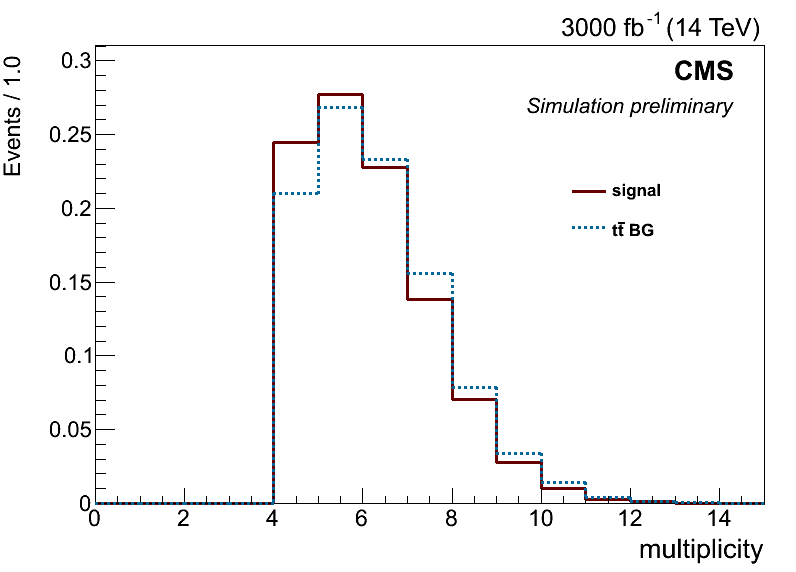
\includegraphics[width=\ww]{figs/Njets20.png}
    \end{minipage}
%    \hspace{\w}
    % fig b
    \begin{minipage}[h!]{\ww}
      \centering
      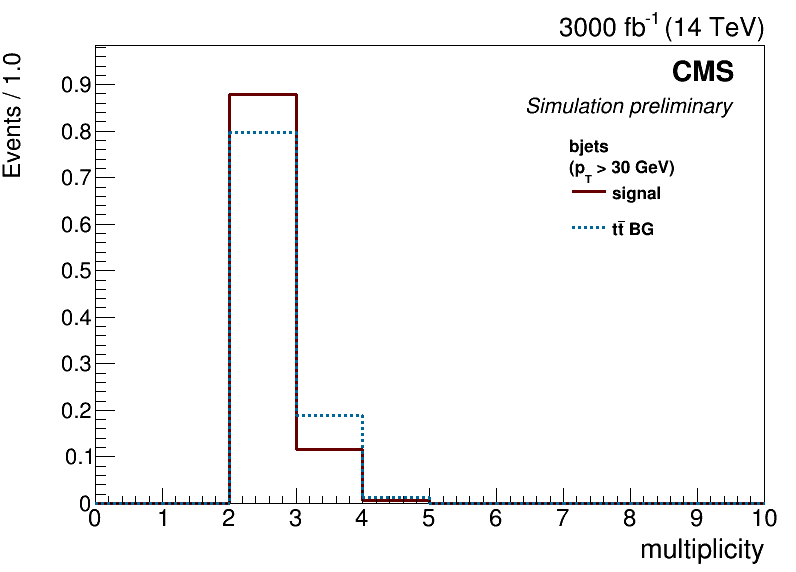
\includegraphics[width=\ww]{figs/Nbjets30.png}
    \end{minipage}
  \vspace{\dd}
  \caption{Multiplicities of $p_T>20$ GeV jets and $p_T>30$ GeV.} \label{multi}
\end{figure*}


% FIGURE: p_T lepton, MET
\begin{figure*}[h]
  % SUBFIGURES
    % fig a
    \begin{minipage}[h!]{\ww}
      \centering
      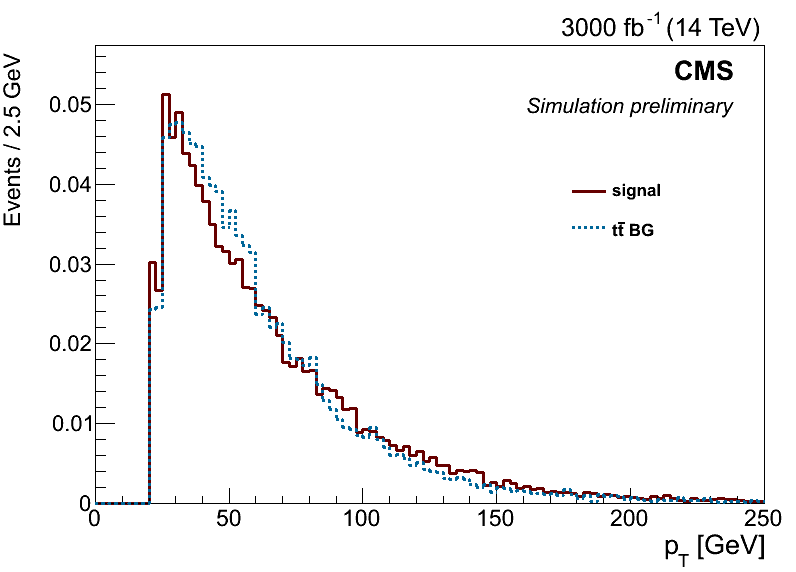
\includegraphics[width=\ww]{figs/leptonPt.png}
    \end{minipage}
%    \hspace{\wb}
    % fig b
    \begin{minipage}[h!]{\ww}
      \centering
      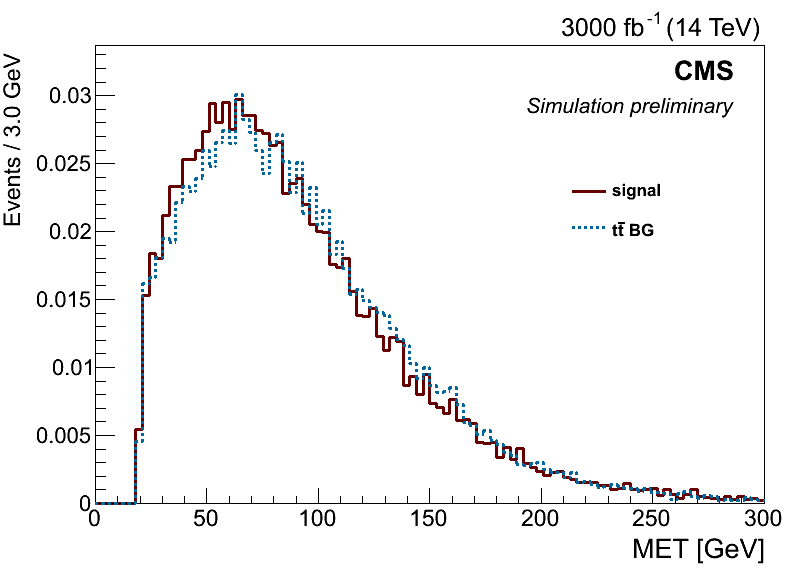
\includegraphics[width=\ww]{figs/MET.png}
    \end{minipage}
  \vspace{\dd}
  \caption{Variables distribution of HH (red) and \tt\ (blue) for the neural network: transverse momentum $p_T$ of the lepton and missing transverse energy \MET.} \label{vars1}
\end{figure*}


%% FIGURE
%\begin{figure*}[h]
%	
%  % SUBFIGURES
%  \begin{subfigure}[b]{17cm}
%    % fig a
%    \begin{minipage}[h!]{\ww}
%      \centering
%      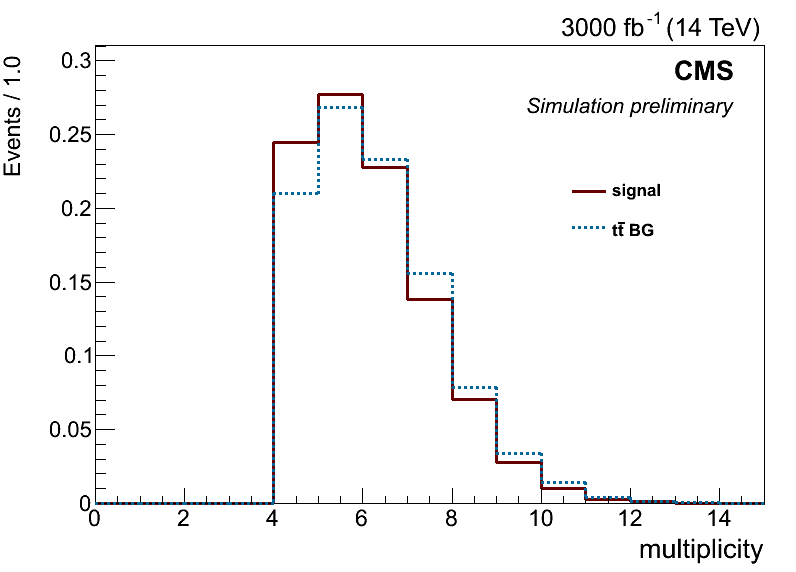
\includegraphics[width=\ww]{figs/Njets20.png}
%    \end{minipage}
%%    \hspace{\w}
%    % fig b
%    \begin{minipage}[h!]{\ww}
%      \centering
%      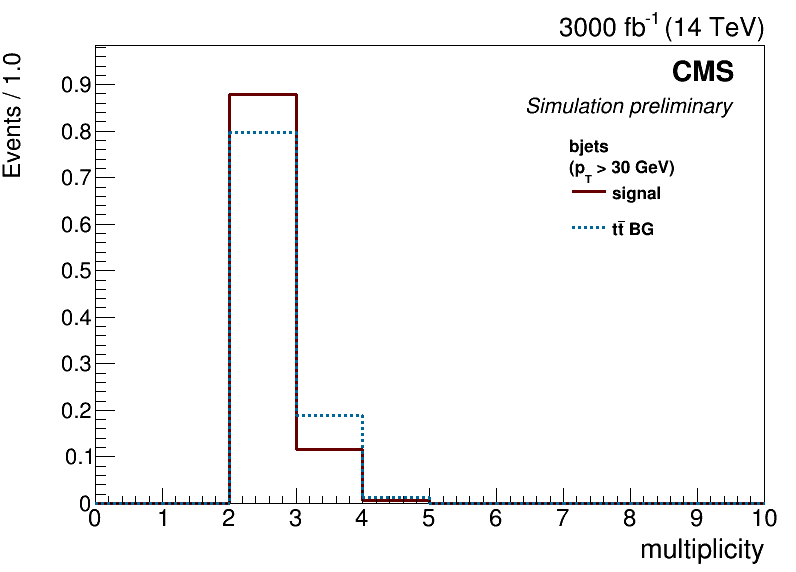
\includegraphics[width=\ww]{figs/Nbjets30.png}
%    \end{minipage}
%  \end{subfigure}
%
%  % SUBFIGURES
%  \begin{subfigure}[b]{17cm}
%    % fig a
%    \begin{minipage}[h!]{\ww}
%      \centering
%      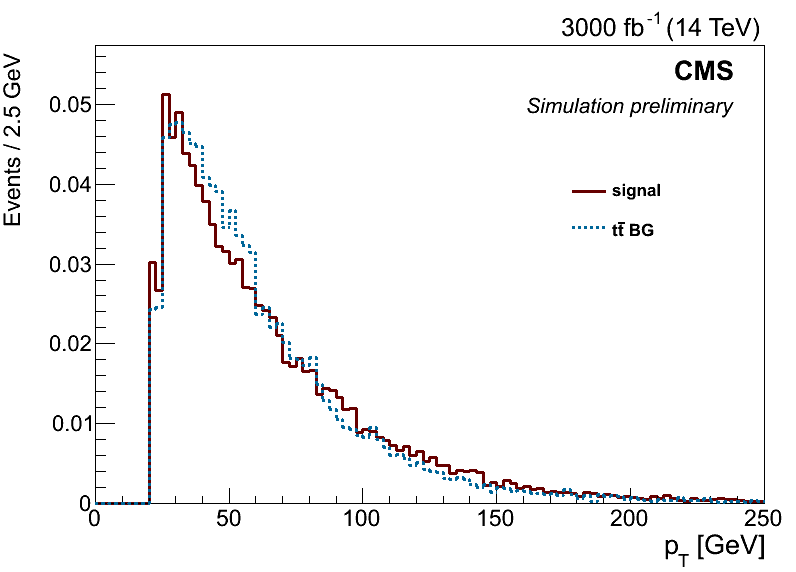
\includegraphics[width=\ww]{figs/leptonPt.png}
%    \end{minipage}
%%    \hspace{\wb}
%    % fig b
%    \begin{minipage}[h!]{\ww}
%      \centering
%      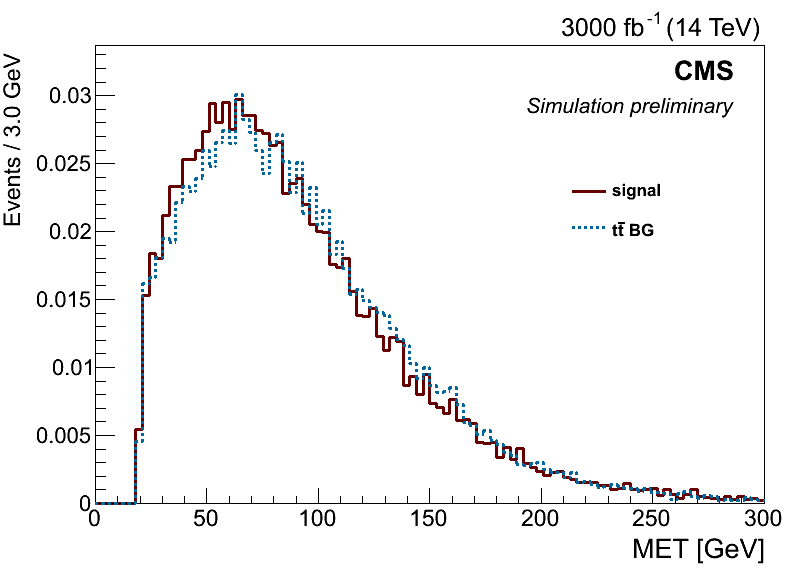
\includegraphics[width=\ww]{figs/MET.png}
%    \end{minipage}
%  \end{subfigure}	
%  \vspace{\dd}
%  \caption{Variables distribution of HH (red) and \tt\ (blue) for the neural network: $p_T>20$ GeV jet multiplicity, $p_T>30$ GeV b-jet multiplicity, transverse momentum $p_T$ of the lepton and missing transverse energy \MET.} \label{vars1}
%
%\end{figure*}



% FIGURE: p_T jets and b-jets
\begin{figure*}[h]
	
  % SUBFIGURES
  \begin{subfigure}[b]{17cm}
    % fig a
    \begin{minipage}[h!]{\ww}
      \centering
      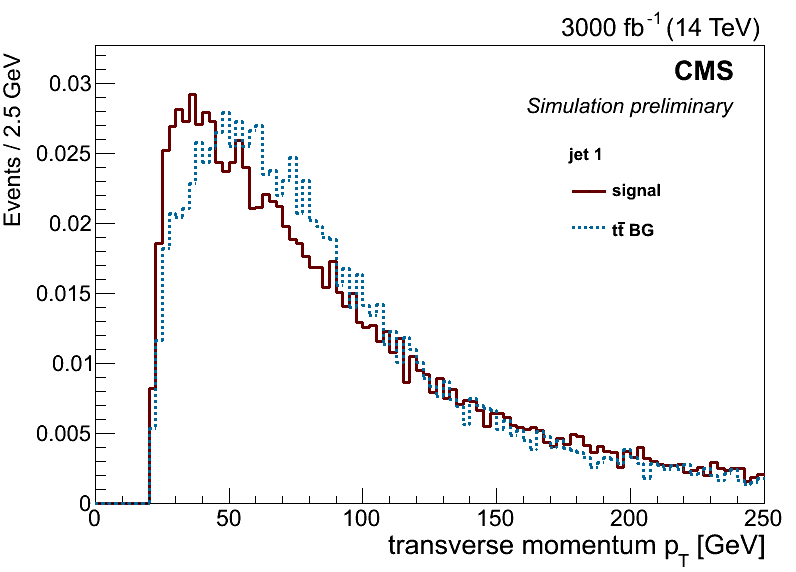
\includegraphics[width=\ww]{figs/jet1Pt.png}
    \end{minipage}
%    \hspace{\w}
    % fig b
    \begin{minipage}[h!]{\ww}
      \centering
      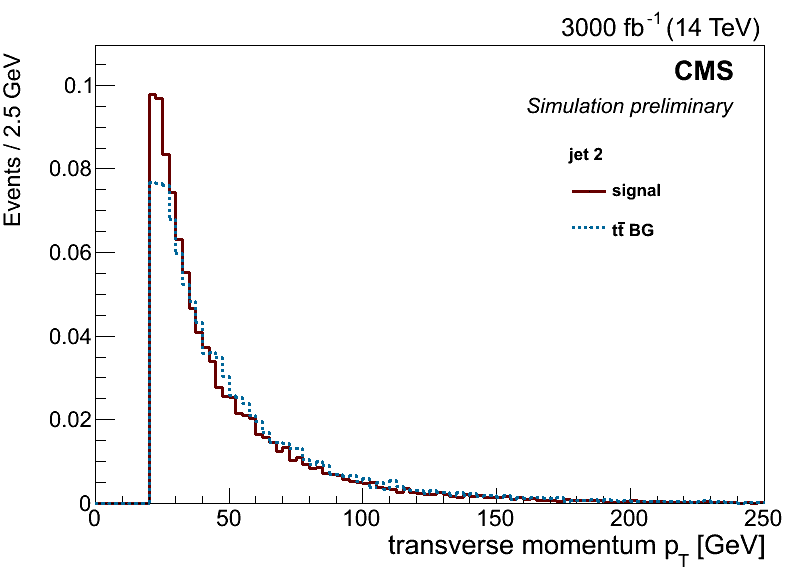
\includegraphics[width=\ww]{figs/jet2Pt.png}
    \end{minipage}
  \end{subfigure}

  % SUBFIGURES
  \begin{subfigure}[b]{17cm}
    % fig a
    \begin{minipage}[h!]{\ww}
      \centering
      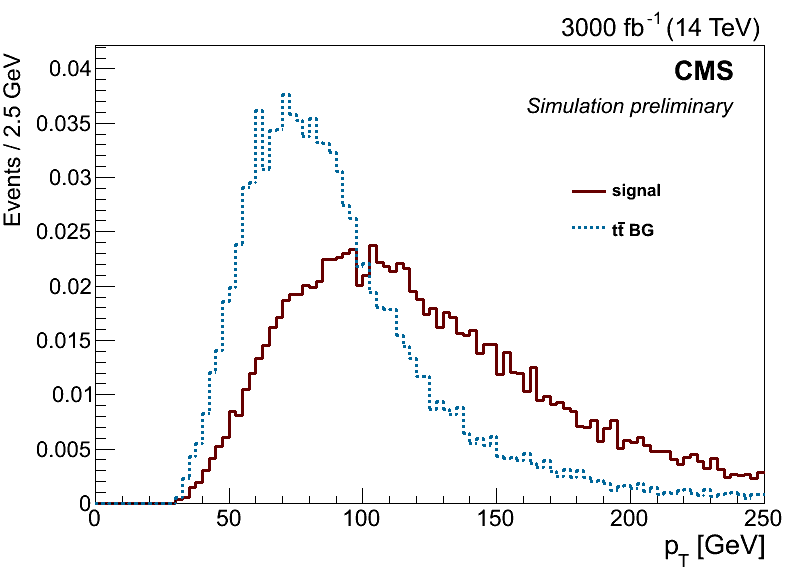
\includegraphics[width=\ww]{figs/bjet1Pt.png}
    \end{minipage}
%    \hspace{\wb}
    % fig b
    \begin{minipage}[h!]{\ww}
      \centering
      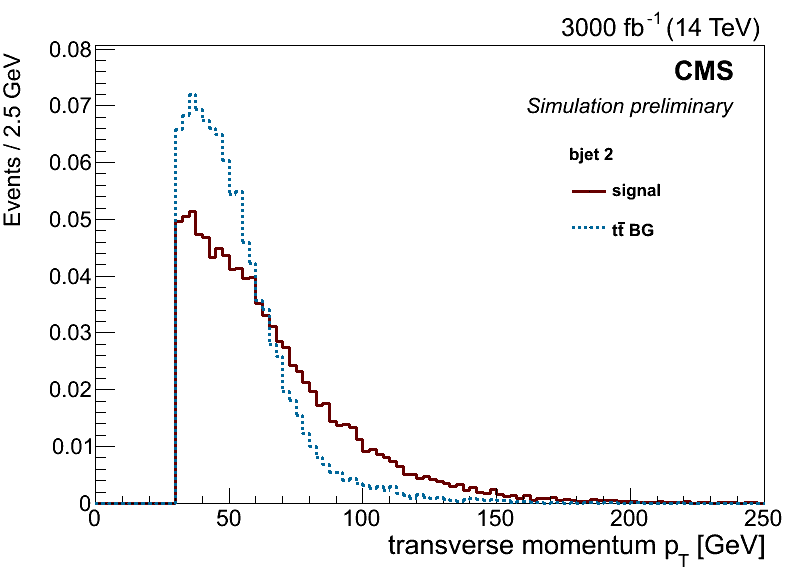
\includegraphics[width=\ww]{figs/bjet2Pt.png}
    \end{minipage}
  \end{subfigure}	
  \vspace{\dd}
  \caption{Variables distribution of HH (red) and \tt\ (blue) for the neural network: transverse momentum $p_T$ for the two leading jets and two leading b-jets.} \label{vars2}

\end{figure*}



% FIGURE: p_T bb, jj, j1l and DeltaPhi_j1lbb
\begin{figure*}[h]
	
  % SUBFIGURES
  \begin{subfigure}[b]{17cm}
    % fig a
    \begin{minipage}[h!]{\ww}
      \centering
      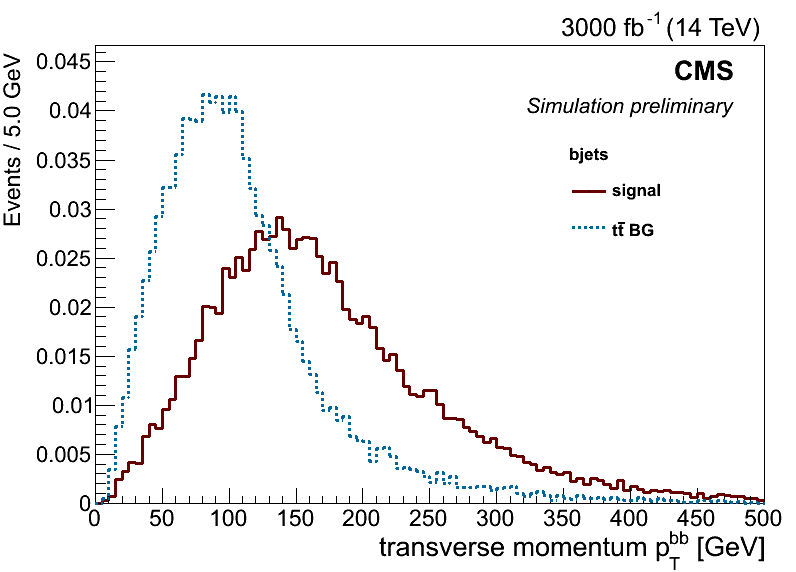
\includegraphics[width=\ww]{figs/Pt_bb.png}
    \end{minipage}
%    \hspace{\w}
    % fig b
    \begin{minipage}[h!]{\ww}
      \centering
      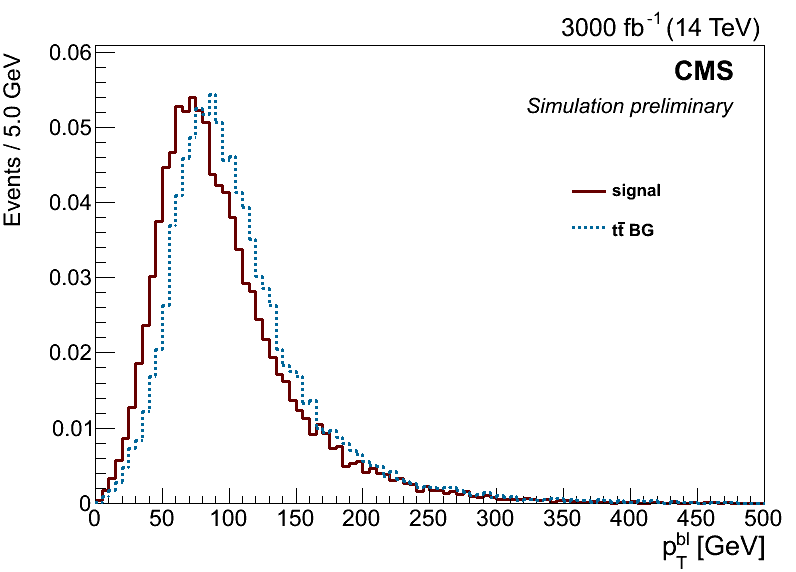
\includegraphics[width=\ww]{figs/Pt_bl.png}
    \end{minipage}
  \end{subfigure}

  % SUBFIGURES
  \begin{subfigure}[b]{17cm}
    % fig a
    \begin{minipage}[h!]{\ww}
      \centering
      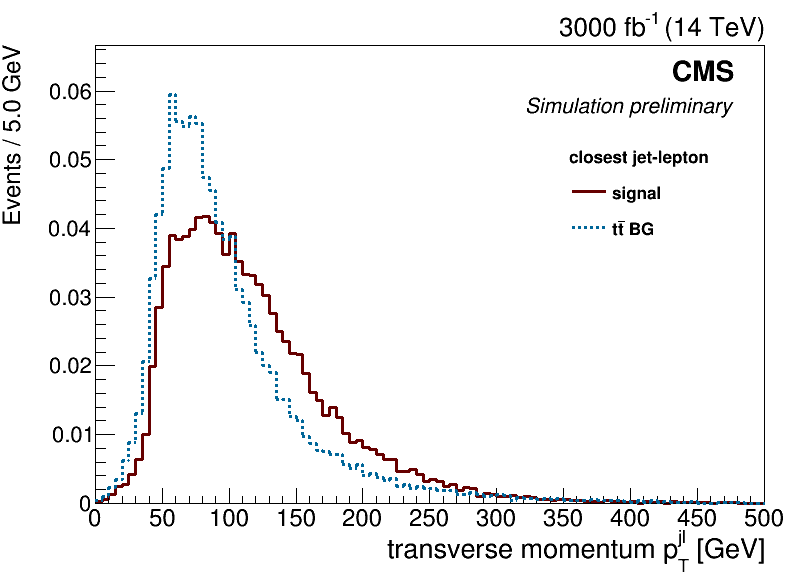
\includegraphics[width=\ww]{figs/Pt_j1l.png}
    \end{minipage}
%    \hspace{\wb}
    % fig b
    \begin{minipage}[h!]{\ww}
      \centering
      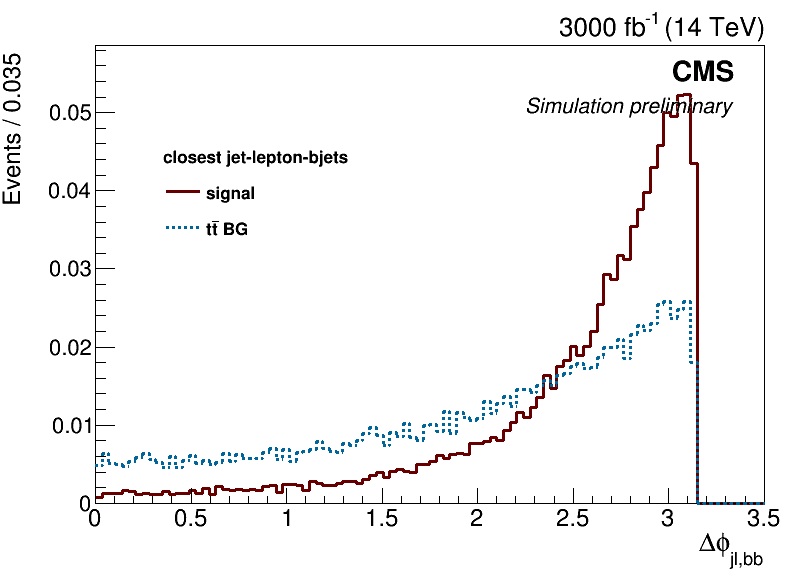
\includegraphics[width=\ww]{figs/DeltaPhi_j1lbb.png}
    \end{minipage}
    \hspace{9mm}
  \end{subfigure}	
  \vspace{\dd}
  \caption{Variables distribution of HH (red) and \tt\ (blue) for the neural network: $p_T^\text{bb}$, $p_T^{jj}$, $p_T^{j_1\ell}$ and $\Delta\phi_{j_1\ell\text{,bb}}$.} \label{vars4}

\end{figure*}



% FIGURE: DeltaR j1l, j2l, b1l, b2l
\begin{figure*}[h]
	
  % SUBFIGURES
  \begin{subfigure}[b]{17cm}
    % fig a
    \begin{minipage}[h!]{\ww}
      \centering
      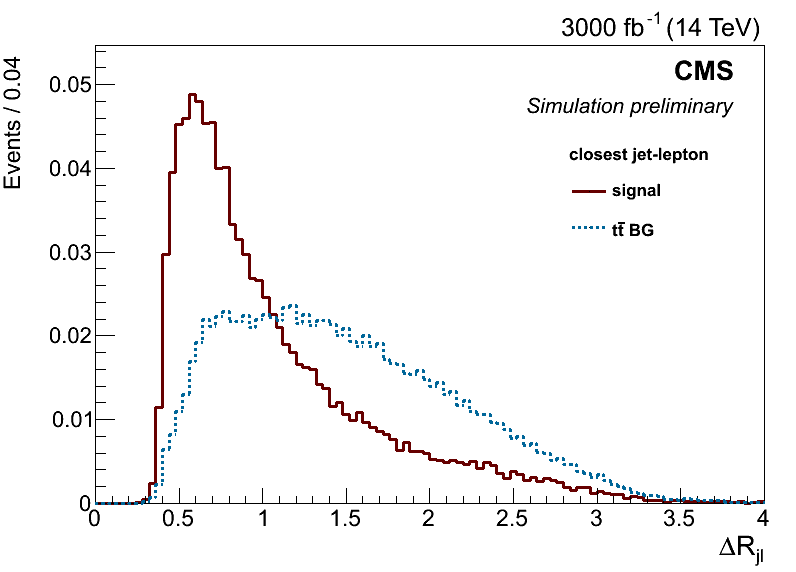
\includegraphics[width=\ww]{figs/DeltaR_j1l.png}
    \end{minipage}
%    \hspace{\w}
    % fig b
    \begin{minipage}[h!]{\ww}
      \centering
      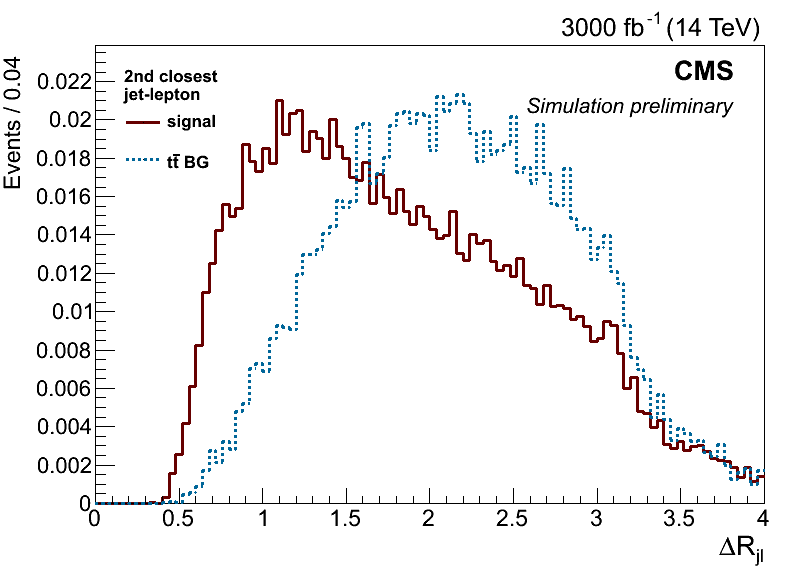
\includegraphics[width=\ww]{figs/DeltaR_j2l.png}
    \end{minipage}
  \end{subfigure}

  % SUBFIGURES
  \begin{subfigure}[b]{17cm}
    % fig a
    \begin{minipage}[h!]{\ww}
      \centering
      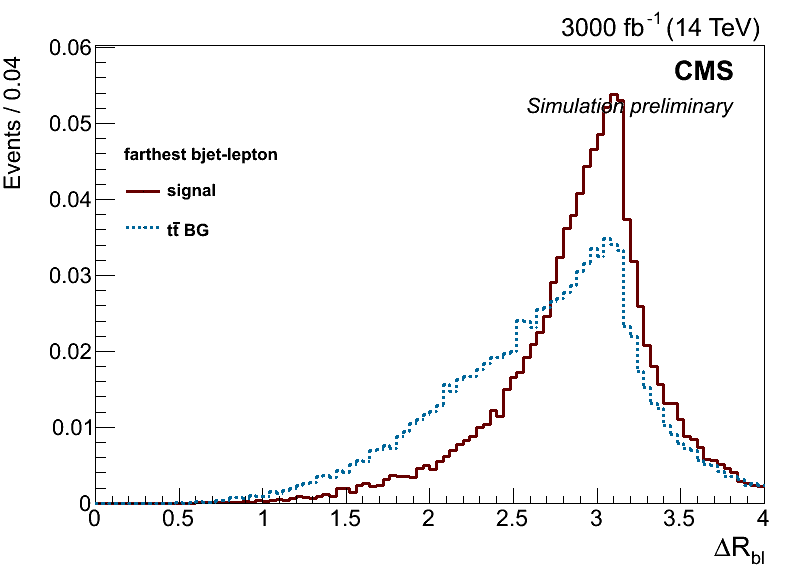
\includegraphics[width=\ww]{figs/DeltaR_b1l.png}
    \end{minipage}
%    \hspace{\wb}
    % fig b
    \begin{minipage}[h!]{\ww}
      \centering
      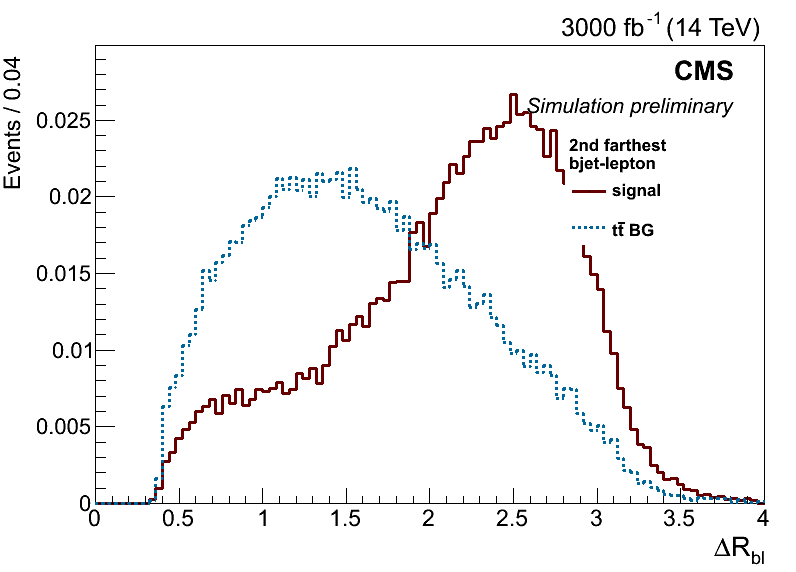
\includegraphics[width=\ww]{figs/DeltaR_b2l.png}
    \end{minipage}
    \hspace{9mm}
  \end{subfigure}	
  \vspace{\dd}
  \caption{Variables distribution of HH (red) and \tt\ (blue) for the neural network: $\Delta R_{j_1\ell}$, $\Delta R_{j_2\ell}$, $\Delta R_{b_1\ell}$ and $\Delta R_{b_2\ell}$.} \label{vars5} %between the lepton and the two closest light jets and between the lepton and two farthest b-jets

\end{figure*}



% FIGURE: DeltaR bb, jj, jjb, jjl
\begin{figure*}[h]
	
  % SUBFIGURES
  \begin{subfigure}[b]{17cm}
    % fig a
    \begin{minipage}[h!]{\ww}
      \centering
      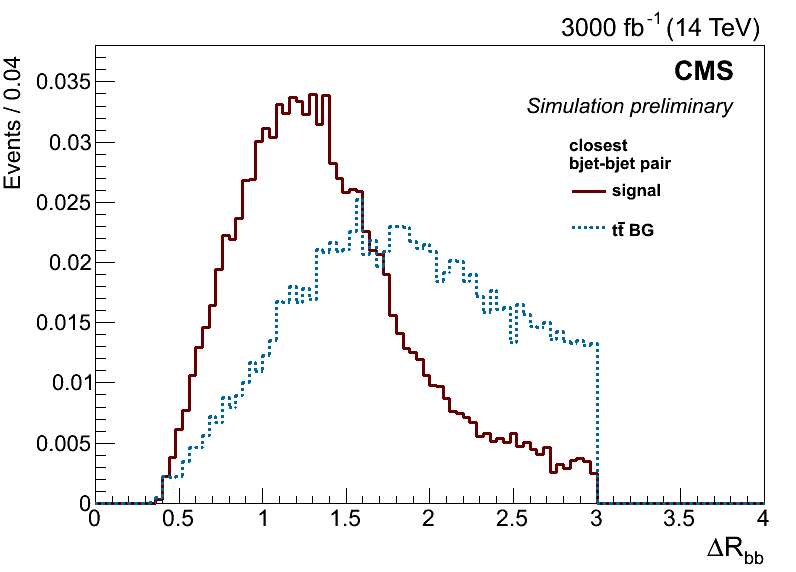
\includegraphics[width=\ww]{figs/DeltaR_bb1.png}
    \end{minipage}
%    \hspace{\w}
    % fig b
    \begin{minipage}[h!]{\ww}
      \centering
      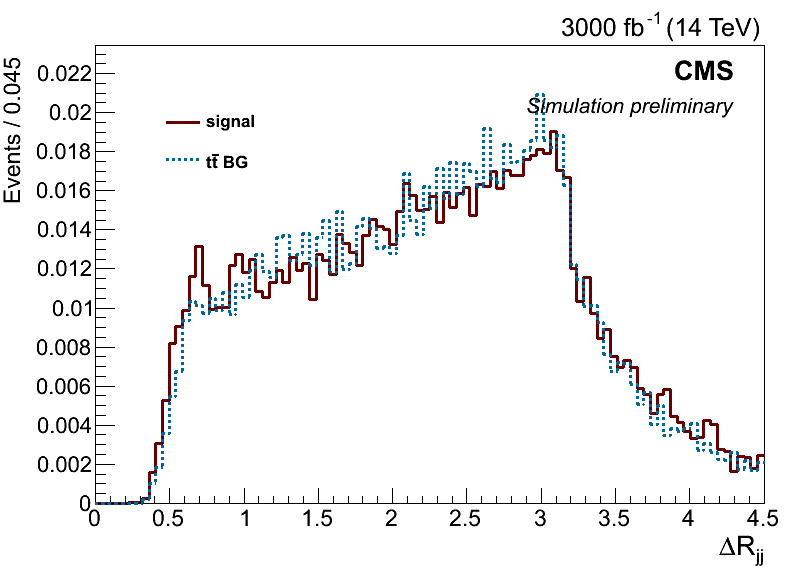
\includegraphics[width=\ww]{figs/DeltaR_jj.png}
    \end{minipage}
  \end{subfigure}

  % SUBFIGURES
  \begin{subfigure}[b]{17cm}
    % fig a
    \begin{minipage}[h!]{\ww}
      \centering
      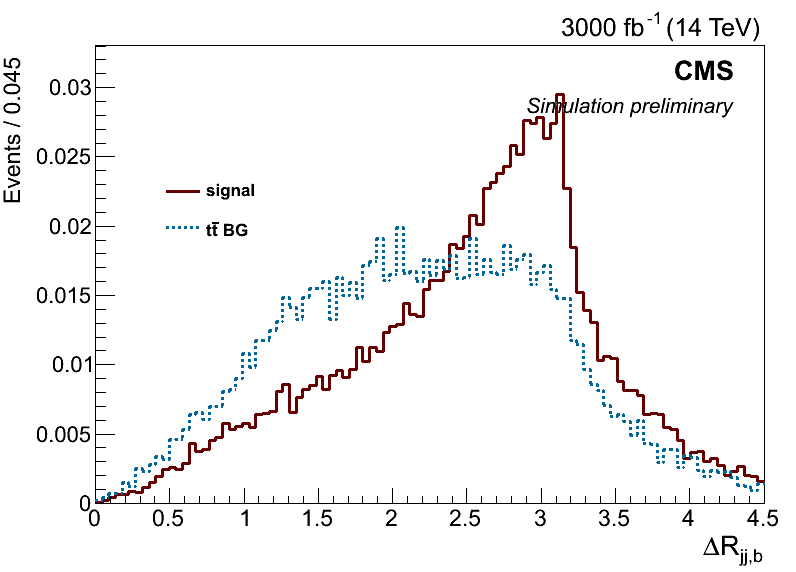
\includegraphics[width=\ww]{figs/DeltaR_jjb.png}
    \end{minipage}
%    \hspace{\wb}
    % fig b
    \begin{minipage}[h!]{\ww}
      \centering
      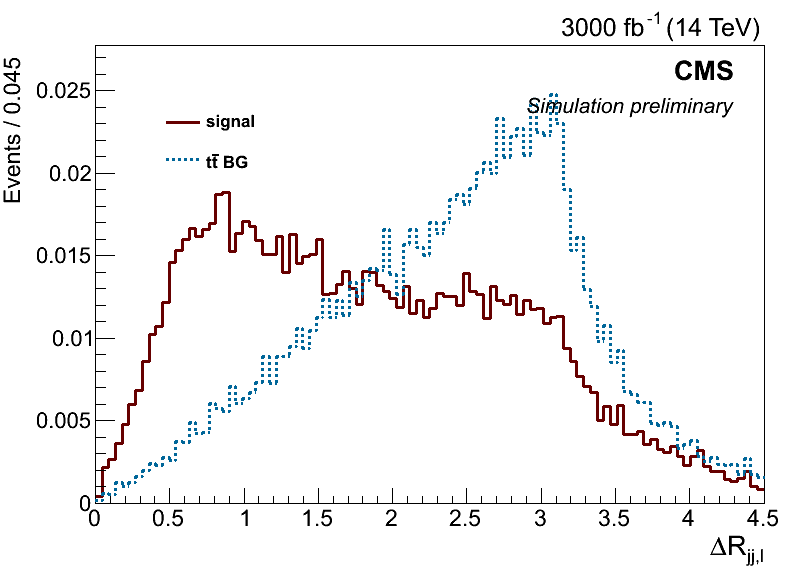
\includegraphics[width=\ww]{figs/DeltaR_jjl.png}
    \end{minipage}
  \end{subfigure}	
  \vspace{\dd} 
  \caption{Variables distribution of HH (red) and \tt\ (blue) for the neural network: $\Delta R_{bb}$, $\Delta R_{jj}$, $\Delta R_{jj,b_1}$ and $\Delta R_{jj,\ell}$.} \label{vars6}

\end{figure*}



% FIGURE: M bb, jjl, jjb, b2lnu
\begin{figure*}[h]
	
  % SUBFIGURES
  \begin{subfigure}[b]{17cm}
    % fig a
    \begin{minipage}[h!]{\ww}
      \centering
      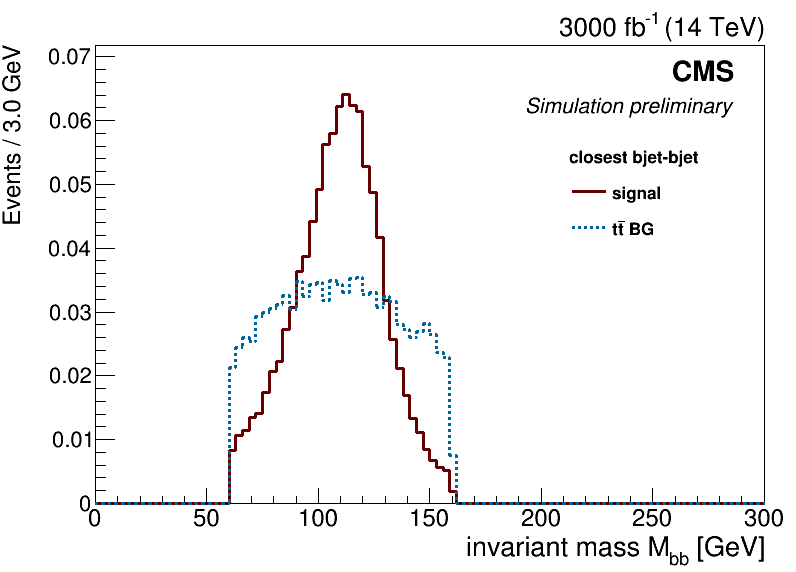
\includegraphics[width=\ww]{figs/M_bb_closest.png}
    \end{minipage}
%    \hspace{\w}
    % fig b
    \begin{minipage}[h!]{\ww}
      \centering
      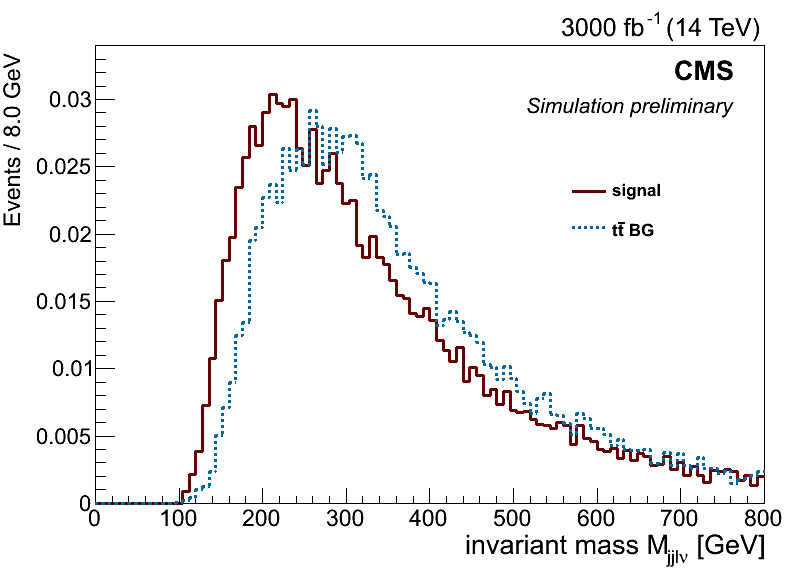
\includegraphics[width=\ww]{figs/M_jjlnu.png}
    \end{minipage}
  \end{subfigure}

  % SUBFIGURES
  \begin{subfigure}[b]{17cm}
    % fig a
    \begin{minipage}[h!]{\ww}
      \centering
      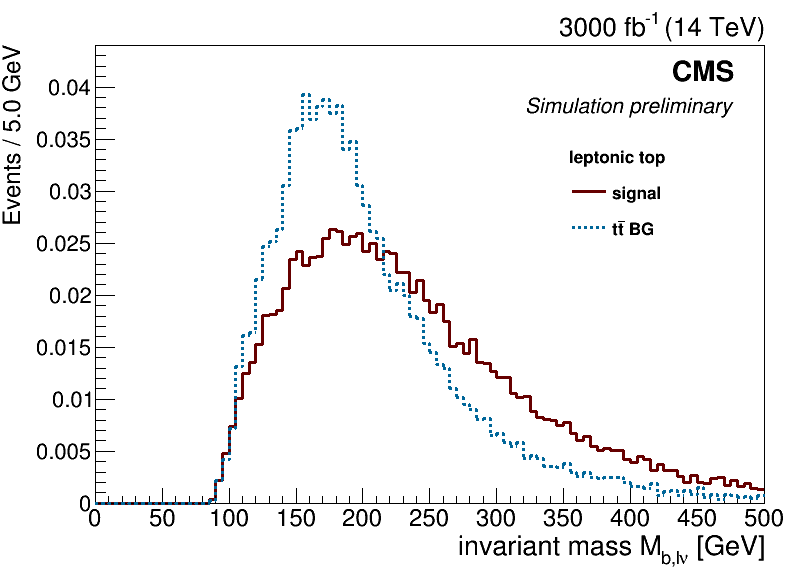
\includegraphics[width=\ww]{figs/M_blnu.png}
    \end{minipage}
%    \hspace{\wb}
    % fig b
    \begin{minipage}[h!]{\ww}
      \centering
      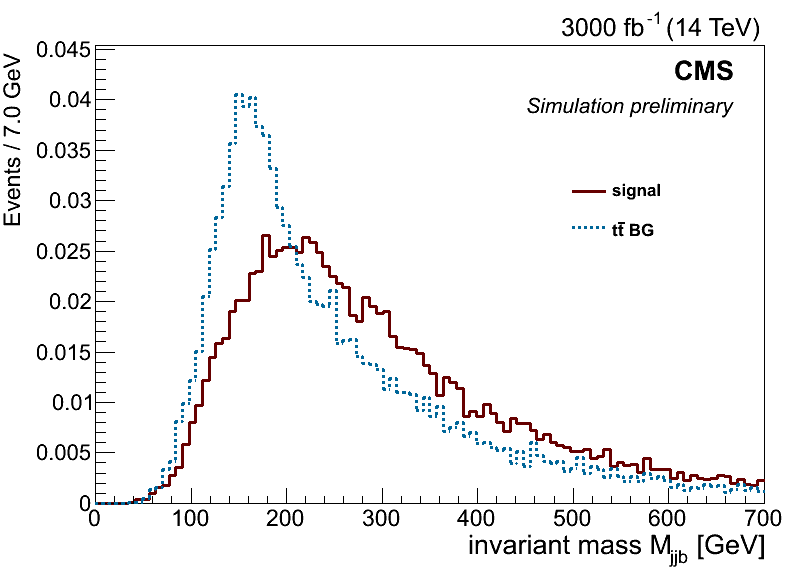
\includegraphics[width=\ww]{figs/M_jjb.png}
    \end{minipage}
    \hspace{9mm}
  \end{subfigure}	
  \vspace{\dd}
  \caption{Variables distribution of HH (red) and \tt\ (blue) for the neural network: Higgs mass reconstructions $M_{\bb}$ and $M_{jj\ell\nu}$ and top mass reconstructions $M_{jj\text{b}_1}$ and $M_{\text{b}_2\text{\lnu}}$.} \label{vars7}

\end{figure*}




% FIGURE: M b2l, j1l and MT
\begin{figure*}[h]
	
  % SUBFIGURES
  \begin{subfigure}[b]{17cm}
    % fig a
    \begin{minipage}[h!]{\ww}
      \centering
      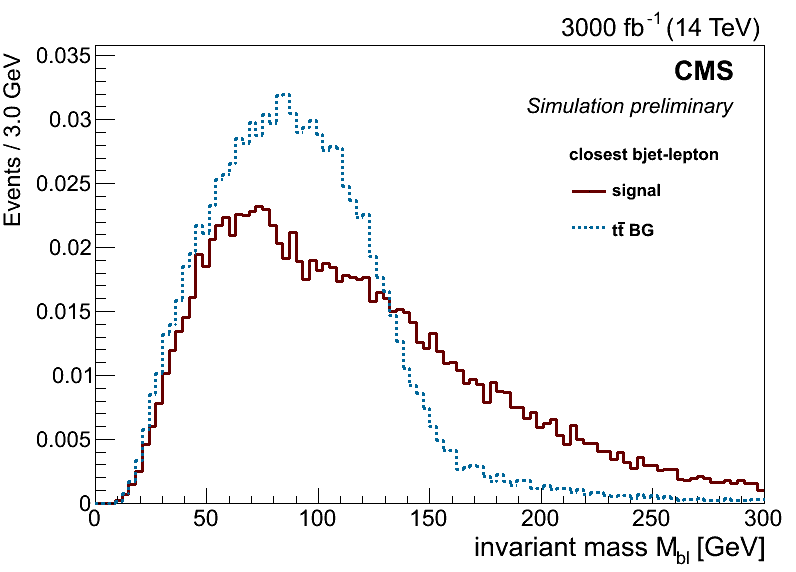
\includegraphics[width=\ww]{figs/M_bl.png}
    \end{minipage}
%    \hspace{\w}
    % fig b
    \begin{minipage}[h!]{\ww}
      \centering
      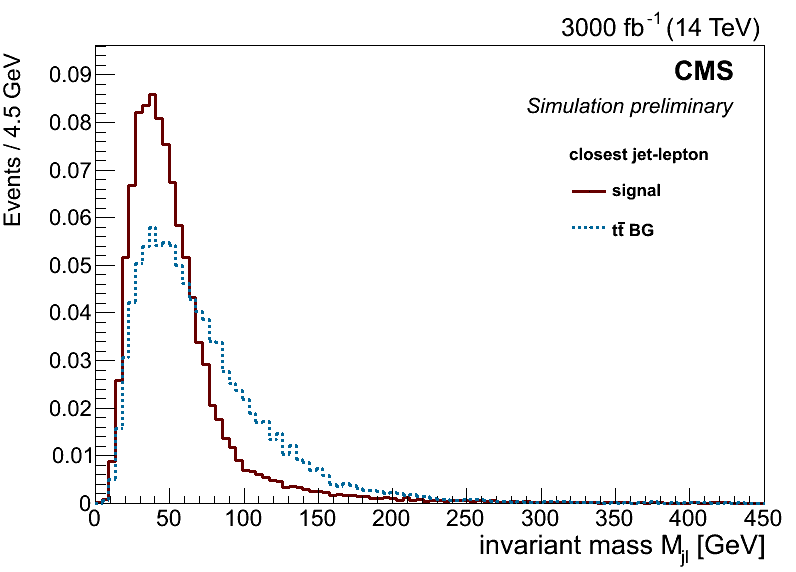
\includegraphics[width=\ww]{figs/M_j1l.png}
    \end{minipage}
  \end{subfigure}

  % SUBFIGURES
  \begin{subfigure}[b]{17cm}
%    % fig a
%    \begin{minipage}[h!]{\ww}
%      \centering
%      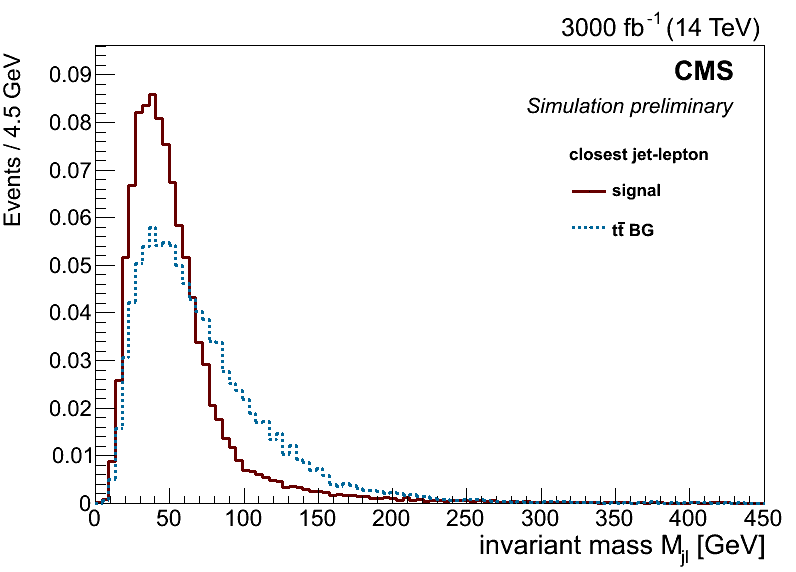
\includegraphics[width=\ww]{figs/M_j1l.png}
%    \end{minipage}
%%    \hspace{\wb}
    % fig b
%    \begin{minipage}[h!]{\ww}
      \centering
      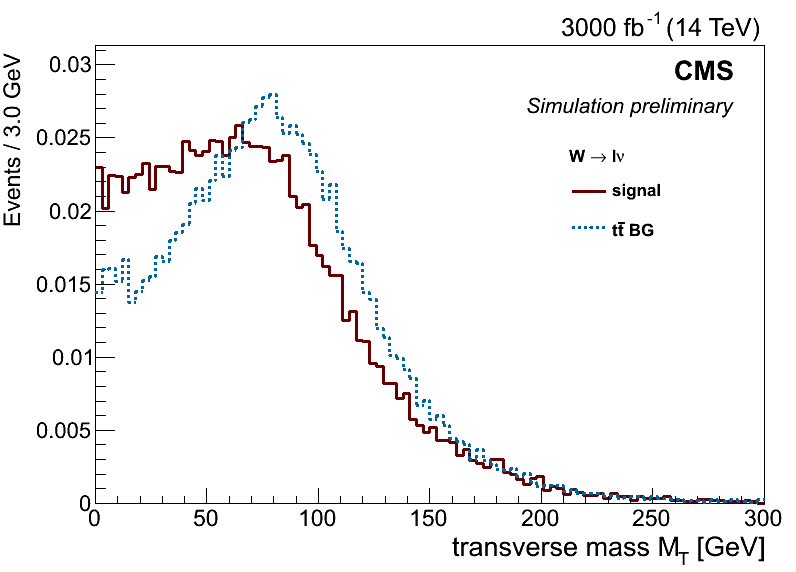
\includegraphics[width=\ww]{figs/MT_lnu.png}
%    \end{minipage}
%    \hspace{9mm}
  \end{subfigure}	
  \vspace{\dd}
  \caption{Variables distribution of HH (red) and \tt\ (blue) for the neural network: $M_{\text{b}_2\text{\l}}$ and $M_T^{\ell\nu}$ (see Eq. \eqref{MT}).} \label{vars8}

\end{figure*}



% FIGURE: MVA output
\begin{figure*}[h] 
	
    % fig a
    \begin{minipage}[h!]{\ww}
      \centering
      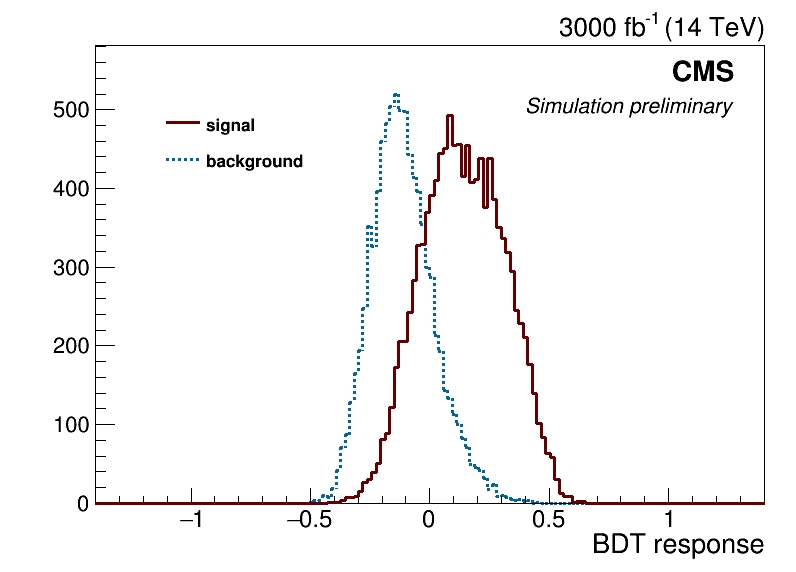
\includegraphics[width=\ww]{figs/BDTBoost1_everything4CleanUp.png}
    \end{minipage}
%    \hspace{\w}
    % fig b
    \begin{minipage}[h!]{\ww}
      \centering
      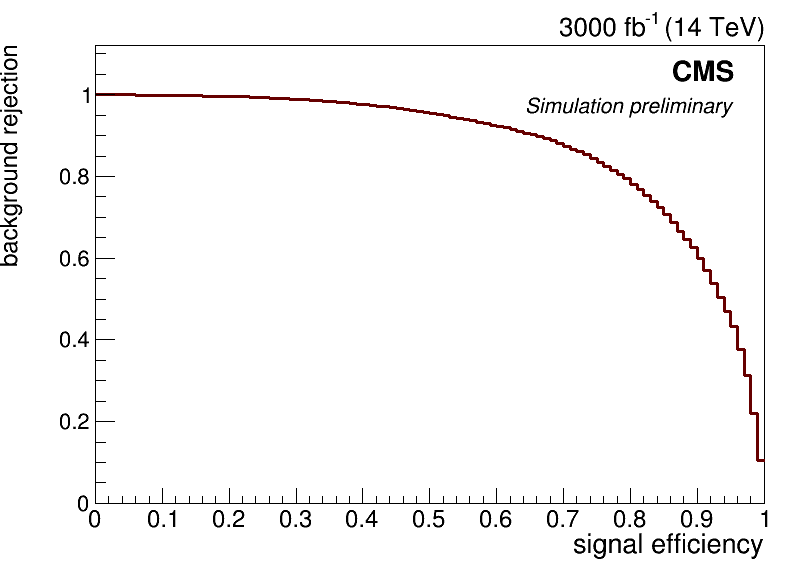
\includegraphics[width=\ww]{figs/BrejvsSeffs_everything4CleanUp_BDTBoost1.png}
    \end{minipage}
  \caption{Final BDT output and background rejection versus signal efficiency.} \label{BDT}

\end{figure*}




% _BRANCHINGRATIOS_HIGGS_BOSON_
%
% https://twiki.cern.ch/twiki/bin/view/LHCPhysics/HiggsEuropeanStrategy2012#SM_Higgs_decay_branching_ratio_M
%    BR(H->bb) = 0,577
%    BR(H->WW) = 0,215
%    BR(H->ZZ) = 0,0264



% _BRANCHINGRATIOS_W_AND_Z_BOSONS_
%
% http://pdg.lbl.gov/2013/listings/rpp2013-list-w-boson.pdf
%    BR(W->qq) = 0,6760
%    BR(W->ev) = 0,1075
%    BR(W->muv) = 0,1057
%    BR(W->tauv) = 0,1125
%
% http://pdg.lbl.gov/2014/listings/rpp2014-list-z-boson.pdf
%    BR(Z->qq) = 0,6991
%    BR(Z->ll) = 0,0337
%    BR(Z->vv) = 0,20/3 = 0,066 ?
%
% Without taus:
%    BR(WW->lvlv) = 0,1075^2 + 2*0,1075*0,1057 + 0,1057^2 = ~ 0,0455
%                 = 4*0,1080^2 = 0,047   % average values
%                 = 4*0,11^2 = 0,0484    % rounded values
%    BR(WW->qqlv) = 2*0,676*(0,1075 + 0,1057)
%                 = 0,2882464 ~ 0,2883
%
% With taus:
%    BR(WW->lvlv) = 0,1075^2 + 0,1057^2 + 0,1125^2
%                   + 2*0,1075*0,1057 + 2*0,1075*0,1125 + 2*0,1057*0,1125
%                 = 0,10608049 ~ 0,1061
%    BR(WW->qqlv) = 2*0,676*(0,1075 + 0,1057 + 0,1125)
%                 = 0,4403464 ~ 0,4403



% _BRANCHINGRATIOS_HH_
%
% Without taus:
%    BR(HH->bbWW->bblvlv) = 2*BR(H->bb)*BR(H->WW)*BR(W->lv)^2
%                         = 2*(0,215*0,577)*(0,1075^2 + 2*0,1075*0,1057 + 0,1057^2)
%                         = 0,01127765149 ~ 0,0113
%    BR(HH->bbWW->bbqqlv) = 2*BR(H->bb)*BR(H->WW)*2*BR(W->qq)*BR(W->lv)
%                         = 2*(0,215*0,577)*2*0,676*(0,1075 + 0,1057)
%                         = 0,0715168143 ~ 0,0715
%
% With taus:
%    BR(HH->bbWW->bblvlv) = 2*BR(H->bb)*BR(H->WW)*BR(W->lv)^2
%                         = 2*(0,215*0,577)*( 0,1075^2 + 0,1057^2 + 0,1125^2
%                           + 2*0,1075*0,1057 + 2*0,1075*0,1125 + 2*0,1057*0,1125 )
%                         = 0,02631963037 ~ 0,0263
%    BR(HH->bbWW->bbqqlv) = 2*BR(H->bb)*BR(H->WW)*2*BR(W->qq)*BR(W->lv)
%                         = 2*(0,215*0,577)*2*0,676*(0,1075 + 0,1057 + 0,1125)
%                         = 0,1092543453 ~ 0,1093
%
% Sample with only H->bb, H->WW combinations
%    2*(0,577)*(0,215) / (2*(0,577)*(0,215)+(0,577)^2+(0,215)^2) ~ 0,3955
%      (0,577)^2 / (2*(0,577)*(0,215)+(0,577)^2+(0,215)^2) ~ 0,5308
%      (0,215)^2 / (2*(0,577)*(0,215)+(0,577)^2+(0,215)^2) ~ 0,0737
%
%



% _BRANCHINGRATIOS_tt_
%
% http://arxiv.org/pdf/1404.3392.pdf
% http://pdg.lbl.gov/2014/reviews/rpp2014-rev-top-quark.pdf
% http://pdg.lbl.gov/2014/tables/rpp2014-sum-quarks.pdf
%    BR(t->bW) = 0,99830 CDF 2014
%    BR(t->bW) = 0,91 PDG 2014
%
% Without taus
%    BR(tt->bbWW->bblvlv) = 0,99830^2 * (0,1075^2 + 2*0,1075*0,1057 + 0,1057^2)
%                         = 0,04529982695 ~ 0,0453 CDF
%                         = 0,03764065614 ~ 0,0377 PDG
%    BR(tt->bbWW->bbqqlv) = 0,99830^2 * 2*0,676*(0,1075 + 0,1057)
%                         = 0,2872671953 ~ 0,2873 CDF
%                         = 0,2386968438 ~ 0,2387 PDG
%
% With taus
%    BR(tt->bbWW->bblvlv) = 0,99830^2 * ( 0,1075^2 + 0,1057^2 + 0,1125^2
%                           + 2*0,1075*0,1057 + 2*0,1075*0,1125 + 2*0,1057*0,1125 )
%                         = 0,1057201229 ~ 0,1057
%    BR(tt->bbWW->bbqqlv) = 0,99830^2 * 2*0,676*(0,1075 + 0,1057 + 0,1125)
%                         = 0,4388504948 ~ 0,4389



% 0,163*2,3/0.0113 = 33,177
% 18899/50789 = 0,372
% 9030*1,85/0,0454/0,37 = 994493
% 9030*1,85/0,37/984500 = 0,04586

% (40*0,0113*3000)*.../51464/(1+sqrt(984500*0,0453*3000*.../50789))
% (40*0,0113*3000)*.../51464/(1+sqrt(984500*0,0453*3000*.../18899))
% (40*0,0715*3000)*.../214888/(1+sqrt(984500*0,2873*3000*.../211952))
% (40*0,0715*3000)*.../214888/(1+sqrt(984500*0,2873*3000*.../182709))
% (0,163*2,3*3000)*.../51464/(1+sqrt(9030*1,85*3000*.../18899))
% (0,163*2,3*3000*715/113)*.../214888/(1+sqrt(9030*1,85*3000*2873/453*.../182709))

%           S = 979907  B = 499600
% stage_0:  S = 51464   B = 50789
% stage_1:  S = 51464   B = 18899
% stage_2:  S = 3181    B = 2023
% stage_3:  S = 2499    B = 331
% stage_4:  S = 214888  B = 211952
% stage_5:  S = 214888  B = 182709
% stage_6:  S = 26511   B = 35223
% stage_7:  S = 20634   B = 15335



\end{document}
